\setcounter{step}{0}

\subsection{ Veterníky }

\begin{ingredient}
  
      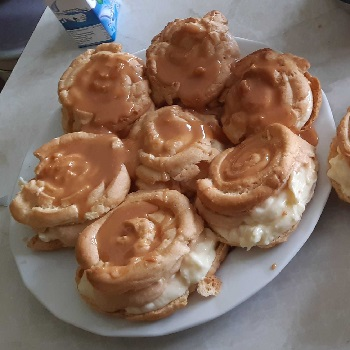
\includegraphics[height=5.5cm]{images/veterniky}
  
  \def\portions{  }
  \textbf{ {\normalsize Ingrediencie (4 porcie):} }

  \begin{main}
      \item 
  \end{main}
  
    \begin{subingredient}{Cesto}
        \item 300 ml voda
        \item 150g palmarín
        \item 150g hladká múka
        \item 4ks vajíčka
    \end{subingredient}
  
    \begin{subingredient}{Plnka 1}
        \item 1-2ks zlatý klas
        \item 750ml mlieko
        \item 1ks vanilkový cukor
        \item 3.5PL práškový cukor
        \item 125ml šľahačka
    \end{subingredient}
  
    \begin{subingredient}{Plnka 2}
        \item 10PL kryštálový cukor
        \item 500ml šľahačka
    \end{subingredient}
  
    \begin{subingredient}{Poleva}
        \item 2.5PL kryštálový cukor
        \item 25ml mlieko
        \item 125g práškový cukor
    \end{subingredient}
  
\end{ingredient}
\begin{recipe}
\textbf{ {\normalsize Príprava:} }
\begin{enumerate}

  \item{Vodu s palmarínom necháme zovrieť a do toho pridáme múku.}
  \item{Miešame 3 minúty nech sa cesto odliepa od hrnca. Necháme vychladnúť.}
  \item{Do cesta primiešame vajíčka po jednom.}
  \item{Na plech vytvarujeme ozdobným vreckom.}
  \item{Pečieme 10 minút na 250C a potom 20 minút na 170C.}
  \item{Ešte horúce veterníky rozrežeme.}
  \item{Pripravíme karamel: }
      \begin{enumerate}
          \item{Do hrnca dáme cukor aj na Plnku 2 aj na Polevu.}
          \item{Časť karamelu pridáme do misky s cukrom na polevu, a zmiešame. (Ak je zmes hustá, pridáme \emph{kúsok} mlieka.)}
          \item{Zvyšok karamelu si odložíme a neskôr pridáme k vymiešaným šľahačkám na Plnku 2.}\end{enumerate}
  \item{Urobíme puding na Plnku 1.}
  \item{Pripravíme šľahačku: }
      \begin{enumerate}
          \item{Vymiešame šľahačku na Plnku 1 aj na plnku 2}
          \item{Po vychladnutí časť šľahačky primiešame do pudingu.}
          \item{Do zvyšku primiešame karamel.}\end{enumerate}
  \item{Naplníme Plnkou 1, Plnkou 2 a polejeme Polevou}

\end{enumerate}
\end{recipe}

\begin{notes}
  
\end{notes}	
\clearpage
